\begin{figure}[H] 
  % \begin{subfigure}[t]{.6\textwidth}
  \begin{minipage}[t]{.55\textwidth}
  \lstset{escapechar=|,basicstyle=\footnotesize\ttfamily}
\begin{lstlisting}[style=boxed, language=Rust]
#[macro_use] mod smack; use smack::*;
extern{fn fib_c(n:u64)->u64;}|\label{code:cextern}|
fn fib(x: usize, cache:&mut Vec<u64>){|\label{code:fib_start}|
  for i in 2..x+1 as usize{|\label{code:iterator}|
    cache[i]=cache[i-1]+cache[i-2];|\label{code:overflow}|
 }
}|\label{code:fib_end}|
fn main(){
  let n=5u64.nondet();|\label{code:nondet}|
  assume!(n > 2);|\label{code:assume}|
  let mut cache=vec![0; n+1];|\label{code:mkvec}|
  cache[0]=0;|\label{code:vectoridx}|
  cache[1]=1;
  fib(n, &mut cache);|\label{code:fncall}|
  let c_result=unsafe{fib_c(n)};|\label{code:ffi}|
  assert!(cache[n]==c_result);|\label{code:assert}|
}
\end{lstlisting}
  \end{minipage}
  % \begin{subfigure}[t]{.4\textwidth}
  \begin{minipage}[t]{.42\textwidth}
  \lstset{language=C,basicstyle=\footnotesize\ttfamily}
    \begin{lstlisting}[style=boxed]
typedef unsigned long ul;
ul fib_c(ul x) {
  ul a = 0, b = 1;
  for (ul i=0; i<x-1; i++) {
    ul tmp = a;
    a = b;
    b = a + tmp;
  }
  return b;
}
\end{lstlisting}
\end{minipage}
%\caption{Example program showing Rust features we support.  It checks the Rust
%implementation of the Fibonacci function (left) against the
%corresponding C implementation (right).}
%\caption{Rust program that checks the equivalence between the Rust (left) and C (right) implementations of the Fibonacci function (\texttt{fib} and \texttt{fib\_c}).}
\caption{Rust program (left) that computes Fibonacci numbers with \texttt{fib} to check its result against the C implementation \texttt{fib\_c} (right).}
\label{fig:crossfib}
\end{figure}


\begin{figure}[H]
  \centering
  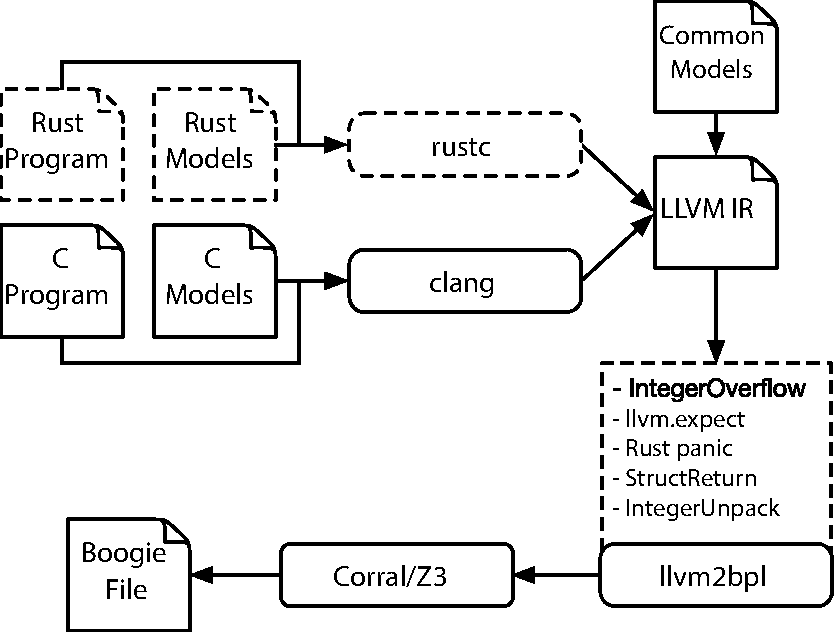
\includegraphics[width=0.99\textwidth]{chap2/figures/RustSmack.pdf}
  \caption{SMACK extensions for Rust.}
  \label{fig:atvatoolflow}
\end{figure}

\begin{figure}[H]\lstset{language=boogie,basicstyle=\scriptsize\ttfamily}
\begin{lstlisting}[style=boxed]
// %x = call {i8,i1} @llvm.uadd.with.overflow.i8(i8 %a,i8 %b)
$a2 := $zext.i8.i16($a);
$b2 := $zext.i8.i16($b);
$x2 := $add.i16($a2, $b2);
$x  := $trunc.i16.i8($x2);
$flag  := $ugt.i16($x2, 255);
assert !$flag;
\end{lstlisting}
\caption{Translation of an unsigned 8-bit checked-addition intrinsic.}
\label{fig:overflow}
\end{figure}

\begin{table}[H]
\caption{Summary of the benchmark suite we developed.}
\vspace{1em}
\begin{center}
\label{tab:benchmarks}
\resizebox{\columnwidth}{!}{
\begin{tabular}{|c|c|c|c|}
\hline
\textbf{Benchmark category} & \textbf{\#Files} & \textbf{LOC} & \textbf{Features demonstrated} \\
\hline
\hline
functions and recursion & 8 & 153 & Function calls, closures, and recursion \\
generics & 6 & 55 & Generic functions, structures, and traits \\
ifc  & 4 & 214 & Information flow control example \\
loops & 4 & 35 & Range-based for loops \\
%other & 4 & Use of nondeterministic values \\
ops & 12 & 171 & Basic operations, overflows \\
%recursion & 4 & Recursive functions \\
structures & 4 & 76 & Creation, passing, and returning of structures \\
vector & 6 & 88 & Dynamic memory management \\
cross-language & 4 & 48 & Combining Rust and C \\
\hline
\end{tabular}
}
\end{center}
\end{table}